\documentclass[runningheads,a4paper]{llncs}

\usepackage{mathtools}
\usepackage{amssymb}
\setcounter{tocdepth}{3}
\usepackage{graphicx}
\usepackage{wrapfig}
\usepackage[caption=false]{subfig}

\usepackage{url}
\usepackage{algpseudocode}
\usepackage{algorithm}
\usepackage{algorithmicx}
  
\newcommand{\keywords}[1]{\par\addvspace\baselineskip
\noindent\keywordname\enspace\ignorespaces#1}

%To economize paper
%\textwidth=190mm
%\textheight=250mm
%\topmargin=-20mm
%\oddsidemargin=-15mm
%\evensidemargin=-15mm


\begin{document}

\algnewcommand\algorithmicswitch{\textbf{switch}}
\algnewcommand\algorithmiccase{\textbf{case}}
\algnewcommand\algorithmicassert{\texttt{assert}}
\algnewcommand\Assert[1]{\State \algorithmicassert(#1)}
% New "environments"
\algdef{SE}[SWITCH]{Switch}{EndSwitch}[1]{\algorithmicswitch\ #1\ \algorithmicdo}{\algorithmicend\ \algorithmicswitch}
\algdef{SE}[CASE]{Case}{EndCase}[1]{\algorithmiccase\ #1}{\algorithmicend\ \algorithmiccase}

\algtext*{EndSwitch}
\algtext*{EndCase}
\algtext*{EndWhile}% Remove "end while" text
\algtext*{EndIf}% Remove "end if" text
\algtext*{EndFor}% Remove "end for" text
\algtext*{EndFunction}% Remove "end function" text

\newtheorem{mydef}{Definition}

\mainmatter  % start of an individual contribution

% first the title is needed
\title{Extended Context-Free Grammars Parsing with Generalized LL}

% a short form should be given in case it is too long for the running head
\titlerunning{ECFG parsing with GLL}

\author{Artem Gorokhov \and Semyon Grigorev}
\authorrunning{Artem Gorokhov, Semyon Grigorev}
% (feature abused for this document to repeat the title also on left hand pages)

\institute{ Saint Petersburg State University\\
            7/9 Universitetskaya nab.\\
            St. Petersburg, 199034 Russia\\
\email{\path|gorohov.art@gmail.com| }
\\
\email{\path|semen.grigorev@jetbrains.com|}
}


\toctitle{Extended Context-Free Grammars Parsing with Generalized LL}
\tocauthor{Artem Gorokhov}
\maketitle

%\tableofcontents

%Authors are invited to submit full papers (not exceeding 12 pages) or short papers (up to 6 pages)

\begin{abstract}

Parsing is important step of static program analysis because it allows to get structural representation of code which necessary for analysis.
One of important source of languages' syntsx specificstion is oficial documentation which often use EBNF to make grammars more compact and expressive.
Moreover, grammar in documentation may be ambiguous.
These facts leads to probelms with parsers creation automation by using parser generators, because the most parsing algorithms and tools reqire transformation to more simple form of grammar (BNF, CNF) and can not handle ambiguose grammars.
There are number of works on ECFG processing without transformation, but no any can handle ambiguous CFG grammar.
On the other hand, there is an generalized LL parsing algorithm, which can handle arbitrary grammars in $O(n^3)$, and LL grammars in $O(n)$, but this algorithm can not handle grammars in EBNF.
We propose modification of generalized LL algorithm which can handle arbitrary grammar in form which close to EBNF (ECFG) without transformations.
Also we implement parser generator based on described algorithm and we demonstarte that proposed modifications allow to get parsing performance improvement.

\keywords{Parsing, GLL, SPPF, EBNF, ECFG, RRPG, Recursive Automata}
\end{abstract}


\section{Introduction}%--------------------------------------------------------------------------------------------------------------------------------------------

Static program analysis usually performed over structural representation of code and parsing is a classical way to get such representation.
Parser generators often used for parser creation automation: these tools allow to create parser from grammar of language which should be specified in appropriate format.
It allows to decrease efforts required for syntax analyzer creation and maintenance.

There are a wide range of parsing techniques and algorithms (CYK, LR(k), LALR(k), LL, etc) and parser generation tools, which based on it. 
The most practical parsing algorifms are LL(k)- and LR(k)-based algorithms.
The LL family is more intuitive than LR and can provide better error diagnostic.
LL(1) is most practical, but not powerful enough, moreover LL(k) for any $k$ is not enough to process some languages: there are LR, but not LL languages.
Also left and hidden left recursion in grammars is a problem for LL-based parsers.
At the same time there is a common problem for both LL- and LR-based tools: handling of arbitrary ambiguous grammars.
All these facts restrict class of grammars which can be handled, which make parser creation difficult. 
In order to solve these problems generalized LL (GLL)~\cite{scott2010gll} was proposed~\cite{scott2010gll}. 
This algorithm handles arbitrary context free grammar, even unambiguous and (hidden)left-recursive.
Worst-case time and space complexity of GLL is cubic in terms of input size and for LL(1) grammars it demonstrates linear time and space complexity.

Extended BNF (EBNF)~\cite{EBNFISO} is a useful format of grammar specification because it allows to make description of language syntax more expressive and compact. 
This formalism often used in documentation, which is one of main source of information for parsers developers.
So, it is necessary to have a parser generator which supports grammar in EBNF.
But classical parsing algorithms requires BNF, and as a result, parser generators requires BNF too.
It is possible to convert from EBNF to BNF but with this conversion we loose the structure of main grammar and resulting trees are for the BNF grammars.

In order to provide ability to process grammar in ELL, ELR~\cite{AttributedELL,ELRR,ECFGparsing,ELLParser,ELL,ECFG,ELALR,ELRParsing} and other can process EBNF but they do not deal with ambiguities in grammars.

At the same time, algorithm for left factorized grammars processing was introduced in~\cite{scott2016structuring}.
Factorization means that there are no two productions for one nonterminal with equal prefixes (look at fig~\ref{fig:ExampleOfFactorization} for example).
Shown, that factorization can reduce memory usage and increase performance which achieved by reusing common parts of rules for one nonterminal.
Prposed idea can be used for processing grammars in EBNF with exception of same effects.

To summarise, it is possible to simplify language description required for parser generation in case a parser generator is based on generalized algorithm which can handle grammars in ECFG.
In this work we present modified generalized LL parsing algorithm which handles grammars in ECFG without transformations.
We show that changes of basic algorithm are very native for GLL nature. 
Also we demonstarte that proposed modifications allow to get parsing performance and memory usage improvement.


%Синтаксический анализ программ это широко известная область, ...
%Проблема в том, что грамматики, используемые в реальной жизни пишутся в форме EBNF. А GLL принимает только BNF.
%Можно проводить преобразование грамматики из EBNF к BNF, но так она разрастается, что, в некоторых случаях, замедляет процедуру разбора.
%Предлагается модификация алгоритма GLL, работающая с грамматиками в форме EBNF.



\section{Extended Contex-Free grammars}%--------------------------------------------------------------------------------------------------------------------------------------------

%Extended Backus-Naur Form~\cite{EBNFISO} is a syntax of expressing context-free grammars. In addition to the Backus-Naur Form syntax it 
%uses such constructions:

%\begin{itemize}
%    \item alternation $\mid$
%    \item option [ ... ]
%    \item repetition \{ ... \}
%    \item grouping ( ... )
%\end{itemize}

%This form is usually used in technical documentation. 
Parser generators widely use Extended CFG form: right parts of productions are regular 
expressions over union alphabet $\Sigma \cup N$. 
\begin{mydef}
An \textbf{extended context-free grammar} (ECFG)~\cite{ECFG} is a tuple ($N$, $\Sigma$, $P$, $S$), where $N$
and $\Sigma$ are finite sets of nonterminals and terminals, $ S\in N$ is the start symbol,
and $P$ (the productions) is a map from $N$ to regular expressions over alphabet $N \cup \Sigma$.
\end{mydef}

It is possible to transform ECFG to CFG~\cite{ELL}, but this transformation leads to grammar size 
increase and change in grammar structure: new nonterminals addition is required during transformation.
As a result, parsing performs not in terms of user defined grammar.
This fact leads to smth... 
There are algorithms for parsing ECFG without transformations, based on different classical algorithms: 
ELL(k) and ELR(k)~\cite{ELL} parsers, Early-style parsers~\cite{!!!}.
Some of them point out a problem with parsing conflicts~\cite{}, and none of them work with arbitrary ECFG.
Generalized parsing algorithms can handle arbitrary grammars and in this paper we
will show how to use them for parsing with arbitrary ECFG.

%Regular expression syntax? Look at ``Towards a Taxonomy for ECFG and RRPG Parsing''



\section{Generalized LL Parsing Algorithm}%--------------------------------------------------------------------------------------------------------------------------------------------

Generalized parsing algorithms (GLL and GLR) was purposed to perform syntax analysis by arbitrary context-free 
grammar. Unlike the GLR, GLL algorithm~\cite{scott2010gll} is rather intuitive and allows to perform better syntax error diagnostic.
As an output of GLL we get Shared Packed Parse Forest(SPPF)~\cite{scott2013gll} that represents all possible derivations of input string.

Work of the GLL algorithm based on descriptors, it allows to handle all posible derivations.
Descriptor is a four-element tuple $(L,i, T, S)$ that can uniquely define state of parsing process. 
$L$ is a grammar slot --- pointer to position in grammar of the form$(S \to \alpha \cdot \beta)$, $i$ --- position in input,
T --- already built SPPF root, $S$ --- current Graph Structured Stack(GSS)~\cite{GSS} node.
%We used efficient GSS described in~\cite{afroozeh2015faster}.

In initial state we have descriptors that describe start positions in grammar and input, dummy tree node and bottom of GSS.
On each step algorithm processes first descriptor in queue and makes actions depending on the grammar and input.
If there are any ambiguity algorithm will queue descriptor for all cases to handle them all. 

There are table based approach~\cite{ragozina} which allows to generate only tables for given grammar instead of full parser code.
The idea is similar to one in original article and main function uses same tree construction and stack processing functions.
Pseudo code can be found in appendix~\ref{GLLCode}. Note that we do not include the check for first/follow sets in this paper.




\section{Extended CFG GLL Parsing}%--------------------------------------------------------------------------------------------------------------------------------------------

In this section we will show an application of Extended Context-Free Grammars(ECFG) in automatons and corresponding GLL-style parsers.

\subsection{Factorization}%--------------------------------------------------------------------------------------------------------------------------------------------

In order to improve performance Elizabeth Scott and Adrian Johnstone offered support of factorised grammars in GLL~\cite{scott2016structuring}. 
The idea is to automatically factorize grammars and use them for parser generation. 

The algorithm creates and queues new descriptors depending on current parse state that we get from unqueued descriptor. 
In case descriptor has been already created it does not add it to queue. For this purpose we have a set of
\textbf{all} created descriptors. Thus reducing a number of possible descriptors decreases the parse time
and required memory.

Factorization decreases the number of grammar slots. 
Consider example from the paper~\cite{scott2016structuring} on fig.~\ref{fig:ExampleOfFactorization}.

\begin{figure}
    \centering
    \subfloat[Production $P_0$]{
        $
        \begin{array}{crcl}
        S::&=& a& a\ B\ c\ d \\
        &|& a& a\ c\ d \\
        &|& a& a\ c\ e \\
        &|& a& a
        \end{array}
        $
    }
    ~
    \subfloat[Production $P_0\prime$]{
        $S::= a\ a\ ( B\ c\ d\ |\ c\ ( d\ |\ e )\ |\ \varepsilon)$
    }
    \caption{Example of factorization}
    \label{fig:ExampleOfFactorization}
\end{figure}
Production $P_0$ factorises to $P_0'$.
Second is much compact and contains much less possible slots, 
so parser creates less descriptors.
It gives significant performance improvement on some grammars.

This idea can also be extended to full ECFG support.
Let us show how to do it.

\subsection{Recursive automata}
The idea of factorisation was evolved to use of automatons and their minimization.

ECFG can be converted to recursive automata~\cite{tellier2006learning}.

\begin{mydef}
    Recursive automaton(RA) $R$ is a tuple $(\Sigma, Q, S, F, \delta)$, where
    $\Sigma$ is a set of terminals,
    $Q$ --- set of states of $R$,
    $S \in Q$ --- start state,
    $F \in Q$ --- set of final states,
    $\delta : Q \times (\Sigma \cup Q) \to Q$ --- transition function.
\end{mydef}

The only difference between RA and FSA is that in RA transition can be labeled either 
by terminal ($\in \Sigma$) or by state ($\in Q$). Further in this peper we will call
transitions by elements from $Q$ as nonterminal transitions and by terminal as terminal transitions.

Right parts of ECFG are regular expressions over alphabet of terminals and nonterminals.
Thus for each right-hand side of grammar productions we can build a finite state automaton 
using Thompson's method~\cite{Thompson:1968:PTR:363347.363387}. 
To transform the set of produced automata we need to eliminate $\varepsilon$-transitions and replace
transitions by nonterminals with transitions labeled by start states of corresponding to nonterminal FSA.
An example of constructed recursive automaton for grammar $\Gamma_{0}$(fig.~\ref{fig:grammarG0})
is given on fig.~\ref{fig:initialAutomatonsForG0}, state 0 is start state.

Decrease of the quantity of the automaton states decreases number of GLL descriptors, as it was with factorization.
Thus to increase performance of parsing we can minimize the number of states in produced automatons.
%without loosing the structure of initial grammar.

First, RA should be converted to deterministic RA using the algorithm for FSA described in ~\cite{aho1974design}.
Then John Hopcroft's algorithm~\cite{hopcroft1971n} can be applied to RA to minimize the number of states.
An example for grammar $G_0$ is shown on fig.~\ref{fig:minimizedAutomatonsForG0}.

%Note: this automatons are not an abstract machines, but just a ``convenient'' representations of grammars.
Note: later we will need a nonterminal names to build a SPPF, for this purpose we define function $\Delta : Q \to N$ where $N$
is nonterminal name.

\begin{figure}
    \centering
    \subfloat[Grammar $G_0$]{
        $
        \begin{array}{crcl}
            S& ::= &(a&|B)\ a \\
            B& ::= &a& \\
        \end{array}
        $
        \label{fig:grammarG0}
    }
    ~
    \subfloat[Initial RA]{
        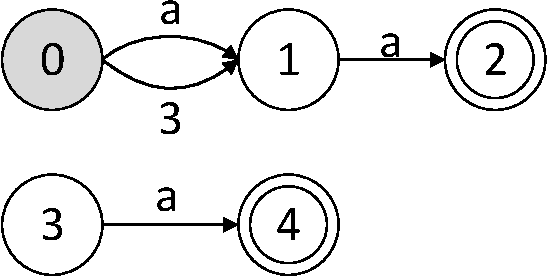
\includegraphics[scale=.48]{pictures/automatonForG0.pdf}
        \label{fig:initialAutomatonsForG0}
    }
    ~
    \subfloat[Minimized RA]{
        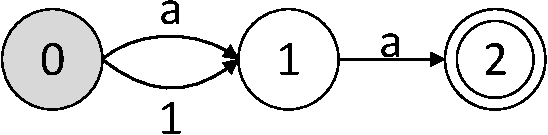
\includegraphics[scale=.46]{pictures/minimizedAutomatonForG0.pdf}
        \label{fig:minimizedAutomatonsForG0}
    }
    \caption{Example of automatons}
    \label{fig:fig1}
\end{figure}

%\begin{figure}
%    \centering
%    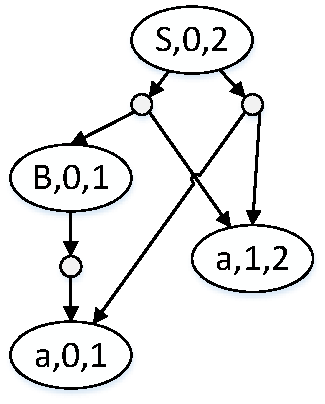
\includegraphics[width=4cm]{pictures/SPPFforG0.pdf}
%    \caption{SPPF for input "aa"}
%    \label{fig:SPPF}
%\end{figure}


\subsection{Input processing}%--------------------------------------------------------------------------------------------------------------------------------------------
An GLL idea is to move through grammar and input simultaneously,
creating multiple descriptors for the case of ambiguity.

Just as we can move through grammar slots we can move through states 
of automaton. Grammar slot in descriptor changes to state in RA.
The problem is that in automaton we have nondeterministic choice because there can be 
many transitions to other states. Consider such significant cases:
\begin{itemize} 
\item there are transition by current input terminal to final state
\item there are transition by current input terminal to state that is not final
\item there are nonterminal transition
\end{itemize}
All of them should be handled and this leads to nondeterminism. 
For the last case we just can call create function for each state.
But for the terminal cases we need to add descriptor that describes
next position to queue without checking it's existence in descriptor elimination set.
Thus we use descriptors queue to handle nondeterminism in states, while original algorithm uses it to 
handle ambiguity in grammars.
%So we need to prevent creation of descriptors for each nonterminal on outgoing edges. We can generate tables that 
%tells us what nonterminals can infer strings that starts with current terminal. And add descriptors only for 
%this edges. Moreover we need to create descriptor for edge that marked with current terminal if such exists.

%In states of parsing we can have a nondeterministic choice because the states of automaton can be final states and outgoing edges can contain nonterminals.
%If there exist outgoing edge that contains current terminal we need to create intermediate node.
%But if the next state is final state we also need to create nonterminal node and call \textbf{pop} function.
%Moreover we need to call \textbf{create} function for edges that contains nonterminal.
%To handle nondeterminism \textbf{parse} function queues new descriptors for all described cases.

\begin{algorithmic}
\Function{add}{$S,u,i,w$}
    \If{$(S,u,i,w) \notin U$}  
        \State $U.add(S,u,i,w)$
        \State $R.add(S,u,i,w)$
    \EndIf
\EndFunction
\end{algorithmic}
Function \textbf{add} queues descriptor if it was not already created.
\begin{algorithmic}    
\Function{create}{$S_{call}, S_{next}, u, i, w$}
    \State $A \gets \Delta(S_{call})$
    \If{($\exists$ GSS node labeled $(A, i)$)}  
    
        \State $v \gets$ GSS node labeled $(A, i)$
        \If{(there is no GSS edge from $v$ to $u$ labeled ($S_{next},w$))}
            \State add GSS edge from $v$ to $u$ labeled ($S_{next},w$)
            \For{($(v, z) \in \mathcal{P} $)}
                \State $(y,N) \gets$ \textbf{getNodes}($S_{next}, u.nonterm, w, z$)
                
                \State $(\_, \_, h) \gets y$
                \State \textbf{add}($S_{next} , u, h, y$)
                
                \If{$N \neq \$$}
                    \State $(\_, \_, h) \gets N$
                    \State \textbf{pop}$(u,h,N)$ 
                \EndIf
            \EndFor
        \EndIf
    \Else
        \State $v \gets$ \textbf{new} GSS node labeled $(A, i)$
        \State create GSS edge from $v$ to $u$ labeled ($S_{next}, w$)
        \State \textbf{add}($S_{call}, v, i, \$ $)
    \EndIf
    \Return{$v$}
\EndFunction
\end{algorithmic}  

Function \textbf{create} is called when we meet nonterminal transition.
It performs necessary operations with GSS and checks if there are already built SPPF for current
input position and nonterminal.
\begin{algorithmic}   
\Function{pop}{$u,i,z$}
    \If{($(u,z) \notin \mathcal{P}$)}  
        \State $\mathcal{P}.add(u,z)$
        \ForAll{GSS edges $(u,S,w,v)$}
            \State $(y,N) \gets$ \textbf{getNodes}($S, v.nonterm, w, z$)
            \If{$N \neq \$$}
                \ \textbf{pop}$(v,i,N)$ 
            \EndIf
            
            \If{$y \neq \$$}
                \ \textbf{add}($S,v,i,y$)
            \EndIf
        \EndFor
    \EndIf
\EndFunction
\end{algorithmic}
\textbf{Pop} function is called when we reach final state. It queues descriptors for all outgoing edges from current GSS node.

\begin{algorithmic}
\Function{parse}{}
    \State $R.add(StartState, new GSSnode(StartNonterminal,0), 0, \$)$
    \While{$R \neq \varnothing $}
    \State{$(C_{S},C_{U},C_{i},C_{N}) \gets R.Get()$}
    \State{$C_{R} \gets \$$}
    
    \If{$(C_{N} = \$) \& (C_{S}$ is final state)}
    \State $eps \gets \textbf{getNodeT}(\varepsilon, C_{i})$  
    \State $(\underline{\hspace{0.25cm}}, N) \gets \textbf{getNodes}(C_{S},C_{U}.nonterm, \$, eps)$
    \State \textbf{pop}$(C_{U},C_{i},N)$ 
    \EndIf
    
    \For{\textbf{each} $transition (C_{S},label,S_{next})$}
        \Switch{$label$}  
        \Case{$Terminal(x)$ where ($x = input[i]$)}
            \State $R \gets \textbf{getNodeT}(x, C_{i})$
            
            \State $(y, N) \gets \textbf{getNodes}(S_{next},C_{U}.nonterm, C_{N}, R)$
            \If{$N \neq \$$}
                \State \textbf{pop}$(C_{U},i+1,N)$ 
            \EndIf
            
            \State $R.add(S_{next}, C_{U}, i + 1, y)$
            
        \EndCase
    
        \Case{$Nonterminal(S_{call})$}
    %\State{$slots \gets pTable[A][input[i]]$}
    %\If{$slots \neq \varnothing$}
            \State \textbf{create}($S_{call}, S_{next}, C_{U}, C_{i}, C_{N}$)
    %\EndIf
    %\ForAll{$L \in slots$}
    %    \State{\Call{add}{L,u,i,\$}} 
    %\EndFor
        \EndCase
        \EndSwitch
        
    \EndFor
    \EndWhile
\EndFunction
\end{algorithmic}

The main function \textbf{parse} handles queued descriptor and checks all transitions from current state to be appropriate
for current input terminal, or calls create function when meets nonterminal transitions.


\subsection{SPPF construction}

First, we should define derivation trees for recursive automatons: it is an ordered tree whose root labeled with start state,
leaf nodes are labeled with a terminals or $\varepsilon$ and interior nodes are labeled with 
nonterminals $A$ and have a sequence of children that corresponds to transition labels of path in 
automaton that starts from the state $\Delta(A)$. More formal. 

\begin{mydef}

Derivation tree of sentence $\alpha$ for the recursive automaton $R=(\Sigma, Q, S, F, \delta)$:%grammar $G=(\Sigma, N, S, P)$:

\begin{itemize}
\item Ordered rooted tree. Root labeled with $\Delta(A)$
\item Leafs are terminals $\in \Sigma$
\item Nodes are nonterminals $\in \Delta(Q)$
\item Node with label $N_i \in \Delta(q_i)$ has children $l_0 \dots l_n (l_i \in \Sigma \cup \Delta(Q))$ iff exists
path
$q_i \xrightarrow[]{l_0} \dots \xrightarrow{l_n} q_m$, $q_m \in F$. 
%for $\omega = l_0 \cdot l_1 \dots\ l_n\in (\Sigma \cup N)^*$ exists $p \rightarrow M \in P$ such that $\omega \in L(M)$
\end{itemize}

\end{mydef}

Automaton is ambiguous if there exist string that have more than one derivation trees. 
We work with arbitrary grammars, thus our RA can be ambiguous and we can define SPPF that can represent all possible derivation trees.
It is similar to SPPF for grammars described in~\cite{scott2013gll}. SPPF contains symbol nodes, packed nodes
and intermediate nodes. 

Packed nodes are of the form $(S, k)$, where $S$ is a state of automaton. 
Symbol nodes have labels $(X, i, j)$ where $X \in \Sigma \cup N \cup \varepsilon$. 
Intermediate nodes have labels $ (S, i, j) $, where $S$ is a state of automaton. $i$ is position in input before leftmost leaf terminal, $j$ --- position after rightmost leaf.

Packed node necessarily has right child --- symbol node, and optional left child --- symbol or intermediate node.
Nonterminal and intermediate nodes may have several packed children. 
Terminal symbol nodes are leaves.

Use of intermediate and packed nodes leads to binarization of SPPF and thus the space complexity is $O(n^{3})$.
%But in grammars slot defines position,
%previous and next symbol, when DFA state tells the position only. Thus we can can construct SPPF using 
%In general, we can't uniquely correspond an original grammar slot to automaton state.
%We can consider example. For the grammar \ref{fig:grammarG0}, automaton will be represented as showed on fig.\ref{fig:automatonForG0}.
%SPPF for input "aa" is on fig.\ref{fig:SPPF}.

%State $1$ can be matched with two grammar slots: $S ::= (a \cdot a)|(b$ $a)$ and $S ::= (a$ $a)|(b \cdot a)$. 
%But SPPF represents WHAT???


\textbf{function} getNodeT$(x,i)$ did not change

We defined function \textbf{getNodes} which can construct two nodes: intermediate and nonterminal (at least one of them, at most both).
It uses modified function \textbf{getNodeP} that takes additional argument: state or nonterminal name. Symbol in returned SPPF node will be this argument's value.
\begin{algorithmic}
\Function{getNodes}{$S, A, w, z$}
    \If{($S$ is final state)}
        \State $x \gets \textbf{getNodeP}(S, A, w, z)$
    \Else
        \State $x \gets \$ $
    \EndIf
    %\Statex
    %\If{$S.outedges = \varnothing$}
    %    \State $y \gets \$$
    %\Else
        \If{$(w = \$) \&$ not ($z$ is nonterminal node and it's extents are equal)}
            \State $y \gets z$
        \Else
            \State $y \gets \textbf{getNodeP}(S, S, w, z)$
        \EndIf
    %\EndIf
    
    \State \Return{$(y,x)$}
\EndFunction   
\end{algorithmic}
\begin{algorithmic}
\Function{getNodeP}{$S, L, w, z$}
    \State $(\underline{\hspace{0.25cm}}, k, i) \gets z$
    
    \If{($w \neq \$$)}
        \State $(\underline{\hspace{0.25cm}}, j, k) \gets w$
    
        \State $y \gets$ find or create SPPF node labelled $(L, j, i)$  
    
        \If{($\nexists$ child of $y$ labelled $(S, k)$)}
            \State $y\prime \gets \textbf{new}$ $packedNode(S, k)$
            \State $y\prime.addLeftChild(w)$
            \State $y\prime.addRightChild(z)$
            \State $y.addChild(y\prime)$
        \EndIf
    
    \Else
        \State $y \gets$ find or create SPPF node labelled $(L, k, i)$ 
        \If{($\nexists$ child of $y$ labelled $(S, k)$)}
            \State $y\prime \gets \textbf{new}$ $packedNode(S, k)$
            \State $y\prime.addRightChild(z)$
            \State $y.addChild(y\prime)$
        \EndIf
    \EndIf
    \State \Return{$y$}
\EndFunction
\end{algorithmic}

\section{Evaluation}

Left factorization vs EBNF

Small demo example (message to Scott)

\begin{figure}[h]
$$
\begin{array}{crcl}
S ::=& A\ A\ A\ A\ A\ A \\
     &|A\ a\ A\ A\ A\ A \\
A ::=& S\ A\ |\ a\ A\ |\ a \\
\end{array}
$$
\caption{Grammar $G_0$.}
\label{testGrammar}
\end{figure}

We have compared our parsers built on factorized grammar and on minimized automatons.
Grammar $G_0$(fig.~\ref{testGrammar}) was used for the tests,
it has long ``common tail'' which is not unified with factorization.
FSA built for this grammar presented on fig.~\ref{dfa}.

\begin{figure}
\centering
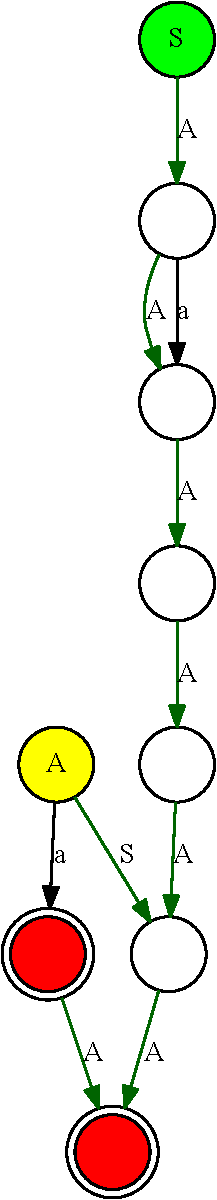
\includegraphics[height=0.95\textwidth,angle=90]{pictures/minimizedDFA.pdf}
\caption{\label{dfa}Minimized automaton for grammar $G_0$}
\end{figure}

Explanation of slots difference: for BNF, for factorized, for ECFG

Description of input. 
Short info about PC.

Note: SPPF construction was disabled while testing.

\begin{table}[h]
\begin{center}
  \begin{tabular}{ | l | l | l | l | l | l | l | l | l | }
\hline
    Length & \multicolumn{2}{ c| }{Time, seconds} & \multicolumn{2}{ c| }{Descriptors} & \multicolumn{2}{ c| }{GSS Nodes} & \multicolumn{2}{ c| }{GSS Edges} \\ \hline
     & factorized & minimized & factorized & minimized & factorized & minimized & factorized & minimized \\ \hline
    100 & 0.206 & 0.127 & 52790 & 38530 & 200 & 200 & 42794 & 28534 \\ \hline
    200 & 1.909 & 1.54 & 215540 & 157030 & 400 & 400 & 175544 & 117034 \\ \hline
    300 & 8.844 & 7.125 & 488290 & 355530 & 600 & 600 & 398294 & 265534 \\ \hline
    400 & 25.876 & 21.707 & 871040 & 634030 & 800 & 800 & 711044 & 474034 \\ \hline
    500 & 60.617 & 51.245 & 1363790 & 992530 & 1000 & 1000 & 1113794 & 742534 \\ \hline
    1000 & 842.779 & 768.853 & 5477540 & 3985030 & 2000 & 2000 & 4477544 & 2985034 \\ \hline
     & \multicolumn{2}{ c| }{Average gain: 19$\%$} & \multicolumn{2}{ c| }{Average gain: 27$\%$} & \multicolumn{2}{ c| }{Average gain: 0$\%$} & \multicolumn{2}{ c| }{Average gain: 33$\%$} \\ \hline
\end{tabular}
\end{center}
\caption{Experiments results.}
\label{expTable}
\end{table}

Table~\ref{expTable} shows that in general minimized version works $19\%$ faster, uses $27\%$ less descriptors and $33\%$ less GSS edges.
Also we use this automaton approach in metagenomic assemblies parsing and it gives visible performance increase.
A bit more discussion on evaluation.


Examples of SPPF.
May be some nontrivial cases: s -> a* a* and so on


\section{Conclusion and Future Work}

Described algorithm implemented in F\# as part of the YaccConstructor project.
Source code available here:~\cite{YaccConstructor}.

Proposed modification can not only increase performance, but also decrease memory usage. 
It is critical for big input processing.
For example, Anastasia Ragozina in her master's thesis~\cite{ragozina} shows that GLL can be used for graph parsing.  
In some areas graphs can be really huge: assemblies in bioinfomatics ($10^8$...).
Proposed modification can improve performance not only in case of classical parsing, but in graph parsing too. 
We perform some tests that shows performance increasing in metagenomic analysis, but full integration with graph parsing and formal description is required.

One of way to specify any useful manipulations on derivation tree (or semantic of language) is an attributed grammars~\cite{!!!}.
YARD supports it but our algorithm is not.
So, attributed grammar and semantic calculation is a future work.

Yet another question is possibility of unification our results with tree languages: our definition of derivation tree for ECFG is quite similar to unranced tree and SPPF is similar to automata for unranced trees~\cite{TATA}.
Theory of tree languages seems more mature than theory of general SPPF manipulations.


\bibliographystyle{abbrv}
\bibliography{bibliography}
\section{Dataset description}\label{section:dataset}

In our evaluation we use dataset which contains the following parts.
{\setlength{\tabcolsep}{0.4em}
	\begin{table}[h]
		\caption{RDFs properties}
		\label{tbl:propRDF}
		\rowcolors{2}{}{lightgray}
		\begin{tabular}{| l | c | c | c | c |}
			\hline
			Name                  & \#V    & \#E     & \#type &\#subClassOf \\
			\hline
			\hline
			atom-primitive				& 291		& 685		& 138	& 122	\\
			univ-bench					& 179		& 413		& 84		& 36		\\
			travel						& 131		& 397		& 90		& 30		\\
			skos							& 144		& 323		& 70		& 1		\\
			people\_pets					& 337		& 834		& 161	& 33		\\
			generations					& 129		& 351		& 78		& 0		\\
			foaf							& 256		& 815		& 174	& 10		\\
			biomed-mesure-prim   	    & 341		& 711		& 130	& 122	\\
			funding						& 778		& 1480		& 304	& 90               \\
			pizza						& 671		& 2604		& 365	& 259              \\
			wine							& 733		& 2450		& 485	& 126              \\
			core							& 1323		& 8684		& 1412	& 178              \\
			pathways						& 6238		& 37196		& 3118 	& 3117             \\
			go-hierarchy					& 45007		& 1960436	& 0		& 490109           \\
			enzyme						& 48815		& 219390		& 14989	& 8163             \\
			eclass\_514en				& 239111		& 1047454	& 72517	& 90962            \\
			go							& 272770		& 1068622	& 58483	& 90512            \\
			\hline
		\end{tabular}
	\end{table}
}

{\setlength{\tabcolsep}{0.4em}
\begin{table*}[h]
\caption{RDFs query $G_2$ (time is measured in seconds and memory is measured in megabytes)}
\label{tbl:tableRDFQ2}
\rowcolors{3}{}{lightgray}
\begin{tabular}{| l | r  r | r  r | r  r | r  r | r  r |}
    \hline

    \multirow{3}{*}{Name}   &   \multicolumn{6}{|c|}{Relational semantics index}	&	\multicolumn{4}{|c|}{Single path semantics index} \\
    \cline{2-11}
    &	\multicolumn{2}{|c|}{RG\_CPU\textsubscript{rel}}	&	\multicolumn{2}{|c|}{RG\_CUSP\textsubscript{rel}}	&	\multicolumn{2}{|c|}{RG\_SPARSE\textsubscript{rel}} &	\multicolumn{2}{|c|}{RG\_CPU\textsubscript{path}}	&	\multicolumn{2}{|c|}{RG\_SPARSE\textsubscript{path}}	 \\
    \cline{2-11}
    &   Time & Mem &  Time     & Mem & Time     & Mem  &  Time     & Mem & Time     & Mem \\
    \hline
    \hline
    atom-primitive          & 0.001 & 0.3  & 0.001 & 0.1 & 0.002 & 0.1   & 0.001 & 0.3  & 0.002 & 0.1   \\
biomedical-mesure-primitive & 0.002 & 0.1  & 0.014 & 2.0   & 0.009 & 0.1   & 0.006 & 0.1  & 0.012 & 0.1   \\
core                        & 0.001 & 0.3  & 0.006 & 0.1 & 0.004 & 0.1   & 0.003 & 0.3  & 0.005 & 0.1   \\
eclass\_514en               & 0.035 & 6.5  & 0.020 & 16.0  & 0.100   & 12.0    & 0.123 & 17.7 & 0.127 & 18.0    \\
enzyme                      & 0.006 & 3.9  & 0.006 & 0.6 & 0.010  & 0.1   & 0.012 & 5.3  & 0.008 & 0.4   \\
foaf                        & 0.001 & 0.1  & 0.004 & 0.1 & 0.002 & 0.1   & 0.001 & 0.1  & 0.003 & 0.1   \\
funding                     & 0.002 & 0.1  & 0.015 & 0.4 & 0.007 & 0.1   & 0.009 & 0.1  & 0.008 & 0.1   \\
generations                 & 0.001 & 0.1  & 0.001 & 0.1 & 0.001 & 0.1   & 0.001 & 0.1  & 0.001 & 0.1   \\
go-hierarchy                & 0.095 & 17.8 & 0.253 & 528.0 & 0.175 & 130.4 & 0.884 & 88.8 & 0.306 & 138.8 \\
go                          & 0.306 & 25.8 & 0.240 & 84.0  & 0.181 & 25.4  & 0.918 & 78.1 & 0.219 & 34.2  \\
pathways                    & 0.005 & 0.2  & 0.005 & 0.4 & 0.004 & 0.1   & 0.017 & 0.5  & 0.003 & 0.1   \\
people\_pets                & 0.001 & 0.1  & 0.007 & 0.1 & 0.004 & 0.1   & 0.001 & 0.1  & 0.005 & 0.1   \\
pizza                       & 0.002 & 0.3  & 0.012 & 0.2 & 0.008 & 0.1   & 0.010  & 0.3  & 0.009 & 0.1   \\
skos                        & 0.001 & 0.1  & 0.001 & 0.1 & 0.001 & 0.1   & 0.001 & 0.1  & 0.002 & 0.1   \\
travel                      & 0.001 & 0.1  & 0.007 & 0.1 & 0.005 & 0.1   & 0.001 & 0.1  & 0.005 & 0.1   \\
univ-bench                  & 0.001 & 0.1  & 0.007 & 0.1 & 0.005 & 0.1   & 0.001 & 0.1  & 0.005 & 0.1   \\
wine                        & 0.001 & 0.3  & 0.006 & 0.1 & 0.004 & 0.1   & 0.002 & 0.3  & 0.004 & 0.1  \\
    \hline
  \end{tabular}
\end{table*}
}

\begin{itemize}
\item The real-world data RDFs provided in CFPQ\_Data dataset\footnote{CFPQ\_Data dataset GitHub repository: \url{https://github.com/JetBrains-Research/CFPQ_Data}. Access date: 12.11.2019.} from~\cite{Mishin:2019:ECP:3327964.3328503}.
\item Geospecies (RDF which contains information about biological hierrarchy\footnote{The Geospecies RDF: \url{https://old.datahub.io/dataset/geospecies}. Access date: 12.11.2019.} and same-generation query over \textit{broaderTransitive} relation) is provided in~\cite{Kuijpers:2019:ESC:3335783.3335791} and integrated in our evaluation with CFPQ\_Data.
\item It was shown in~\cite{Mishin:2019:ECP:3327964.3328503} that matrix-based algorithm is performant enough to handle bigger RDFs than those used in the initial datasets, such as~\cite{RDF}.
So, we add several big RDFs to CFPQ\_Data and use them in our evaluation.
New RDFs: \textit{go-hierarchy, go, enzime, core, pathways} are from UniProt database\footnote{Protein sequences data base: \url{https://www.uniprot.org/}. RDFs with data are avalable here: \url{ftp://ftp.uniprot.org/pub/databases/uniprot/current_release/rdf}. Access date: 12.11.2019}, and \textit{eclass-514en} is from eClassOWL project\footnote{eClassOWL project: \url{http://www.heppnetz.de/projects/eclassowl/}. eclass-514en file is available here: \url{http://www.ebusiness-unibw.org/ontologies/eclass/5.1.4/eclass_514en.owl}. Access date: 12.11.2019.}.
\end{itemize}

The properties of the RDFs from the dataset are given in table \ref{tbl:propRDF}. 
Geospecies RDF contains 450609 vertices, 2311461 edges, and 20867 edges labeled by \textit{broaderTransitive}.
Note that while the number of edges labeled by \textit{broaderTransitive} is equal to provided in~\cite{Kuijpers:2019:ESC:3335783.3335791}, the total number of vertices and edges is bigger. It is because we naively convert each triple from RDF to edge in the graph, while J. Kuijpers et al. use special \textit{neosemantics}\footnote{Neosemantix is an RDF processing plugin for Neo4j. Web page: \url{https://neo4j.com/labs/nsmtx-rdf/}. Access date: 30.03.2020.} plugin which can, for example, handling multivalued properties accurately.  

The variants of the \textit{same-generation query}~\cite{FndDB} are used in almost all cases because it is an important example of real-world queries that are context-free but not regular.
So, variations of the same generation query are used in our evaluation.
All queries are added to the CFPQ\_Data dataset.

We use two queries over \textit{subClassOf} and \textit{type} relations.
The first query is the grammar $G_1$:
\[
 \begin{array}{lcl}
   s  \rightarrow \textit{subClassOf}^{\ -1} \ s \ \textit{subClassOf}   & \quad & s  \rightarrow \textit{type}^{\ -1} \ s \ \textit{type}     \\
   s  \rightarrow \textit{subClassOf}^{\ -1} \ \textit{subClassOf}       & \quad & s  \rightarrow  \textit{type}^{\ -1}  \ \textit{type}

 \end{array}
 \]
The second one is the grammar $G_2$: \[s \rightarrow \textit{subClassOf}^{\ -1} \ s \ \textit{subClassOf} \mid \textit{subClassOf}\]

For geospecies we use same-generation query \textit{geo} from the original paper~\cite{Kuijpers:2019:ESC:3335783.3335791}: \[s \rightarrow \textit{broaderTransitive} \ s \ \textit{broaderTransitive}^{\ -1} \]
\[s \rightarrow \textit{broaderTransitive}  \ \textit{broaderTransitive}^{\ -1} \]


\section{Evaluation Details}

Results for RDFs querying with $G_2$ grammar are presented in table~\ref{tbl:tableRDFQ2}.
We can see, that for small graphs time for both relational and single-path querying are similar for CPU and GPGPU versions, but for bigger graphs (\textit{go} and \textit{go-hierarchy}, for example) GPUPU version is more performant than CPU one.

\balance


\end{document}
